\section{Results}

\subsection{Idea Forest}

Hierarchical clustering yielded an idea forest composed of 3007 instances, 1213 unique ideas, 335 category trees, and 129 non-singleton category trees. In general, category trees were shallow, with a maximum tree height of 5. The number of nodes within a category tree ranged from 1 to X, with the distribution of values roughly following a Poisson distribution. The number of instances per node (denoting equivalent response instances) also roughly follows a Poisson distribution, with number of instances ranging from X to Y.

\begin{table}
	\begin{tabular}[h!]{r | l l l l l l l}
	\textbf{number condition} & 5 & 10 & 20 & 50 & 75 & 100 & all \\ \hline \hline
	HITs & 57 & 47 & 23 & 10 & 10 & 10 & 146\\
	instances & 293 & 471 & 453 & 500 & 634 & 855 & 3007\\
	ideas & 171 & 249 & 278 & 341 & 443 & 177 &1212\\
	category trees & 72 & 79 & 93 & 114 & 172 & 177 &321\\
	non-singleton trees & 28 & 34 & 40 & 48 & 49 & 61 &92\\
	\end{tabular}
\end{table}

% are also roughly poisson distributed (Table TAB). In keeping with the findings for height, trees found in the upper number conditions are smaller than trees found in the lower conditions. The precipitous drop in median tree size suggests that in the largest condition, participants are finding rare ideas with only a few variants and less than 14 instances.

% \begin{table}
% \begin{tabular}[h!]{r | l l l l l l l}
% 	\textbf{number condition} & 5 & 10 & 20 & 50 & 75 & 100 & all \\ \hline \hline
% 	number of nodes& \\ \hline
%     median &5&5&4&3&2&2&2 \\
% 	first quartile &2&2&1&1&1&1&1 \\
% 	third quartile &17&17&14&10&5&5&5 \\
% 	number of instances& \\ \hline
% 	median &14&14&12&10&4&4&4 \\
%     first quartile &4&4&4&2&1&1&1 \\
% 	third quartile &47&45&30&23&13&13&13 \\
% 	\end{tabular}
% 	\caption{Number of ideas and instances in trees}
% \end{table}

% \begin{figure}[h!]
%     \centering
%     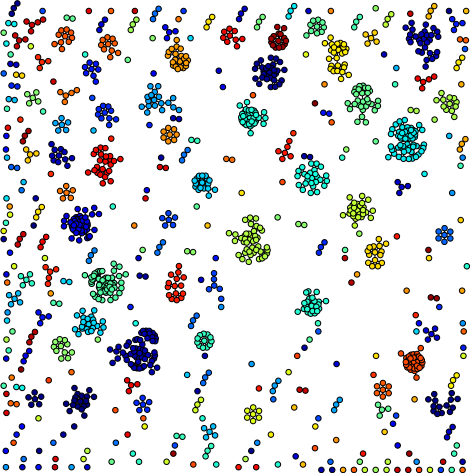
\includegraphics[width=0.9\columnwidth]{idea_forest}
%     \caption{Idea Forest}
% \end{figure}

% The height of category trees follows a roughly Poisson distribution, with the maximum tree height observed at 5. Summary statistics across condition are in table TAB. The third quartile drops as the number condition increases. While the upper conditions still discover categories trees with heights as great as 5, they generate many more "short" trees. This suggests that the ideas generated in the upper conditions are less common.

% \begin{table}
% 	\begin{tabular}[h!]{r | l l l l l l l}
% 	\textbf{number condition} & 5 & 10 & 20 & 50 & 75 & 100 & all \\ \hline \hline
% 	median & 2 & 2 & 2 & 2 & 2 & 2 & 2\\
% 	first quartile & 2 & 2  & 1 & 1 & 1 & 1 & 1\\
% 	third quartile & 3 & 3 &3 &3 &2 &2 & 2\\
% 	\end{tabular}
% 	\caption{Category tree height}
% \end{table}

\subsection{Rates of Idea and Category Production}
The idea forest allows us to model the rate at which new ideas and new categories of ideas are produced, testing hypotheses 1 and 2 (i.e., rates of new ideas and categories of ideas will diminish over time, and will do so differentially per condition).

Figure FIG shows the cumulative count of new ideas as a function of the number of instances gathered in the experiment. For reference, a perfect ``1:1'' idea generation line is also plotted.

We model this quantity using the following logarithmic model:

TODO: num_of_new_ideas = b0 + b_cond * log(x_scale * x + x_trans)

In our model, we assume b0, x_scale, and x_trans do not vary between conditions, while b_cond (essentially, a scaling factor) varies on a per-condition basis. We fit the parameters to the data using a Bayesian approach [REF Kruschke], using the STAN modeling software to perform the actual fit [REF STAN]. The resulting posterior distributions for the parameters allow us to determine whether the conditions are significantly different from one another by comparing whether the posterior distributions' highest density intervals (HDIs) overlap or not. In our analyses, we use an HDI of 95\%.

Analysis of the b_cond HDIs reveals that there are no significant differences between the 5 and 10 conditions, with all other conditions significantly different from one another except for the 50 and 100 conditions.

Taking the derivative of the models allows us to examine the same data, but as rates at which new ideas are produced. As expected, rates of new ideas quickly taper off as a function of the number of ideas received.

\begin{figure}[h!]
    \centering
    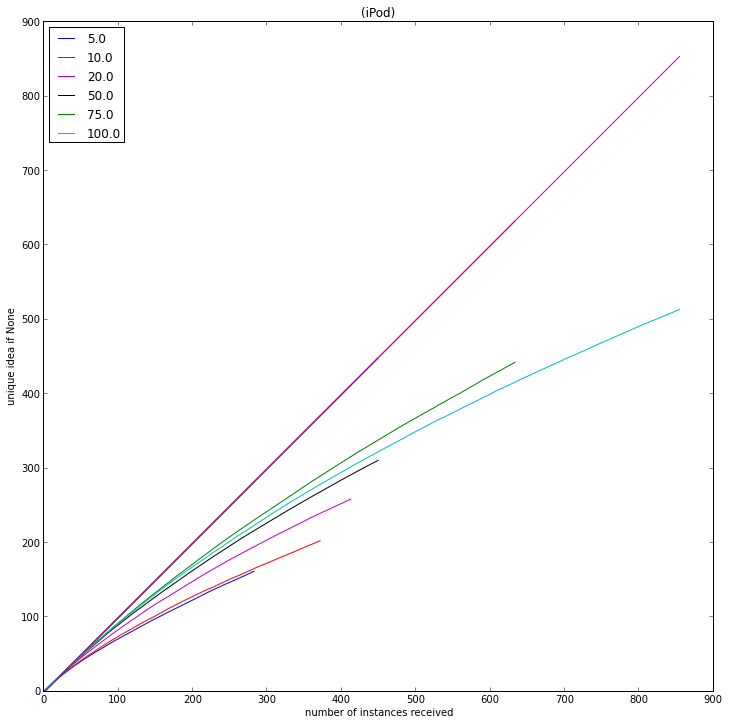
\includegraphics[width=0.9\columnwidth]{ideas_over_time}
    \caption{Cumulative idea count}
\end{figure}

\begin{figure}[h!]
    \centering
    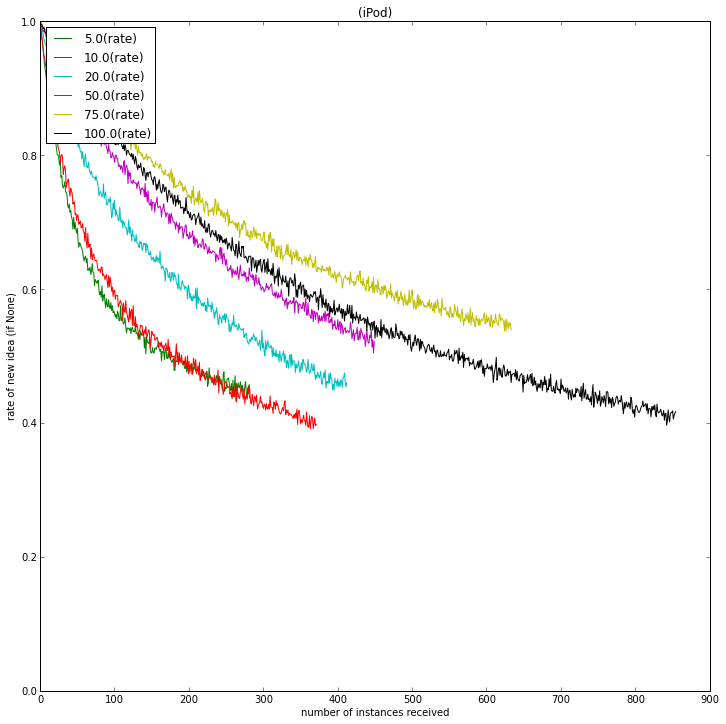
\includegraphics[width=0.7\columnwidth]{rate_new_idea_over_time}
    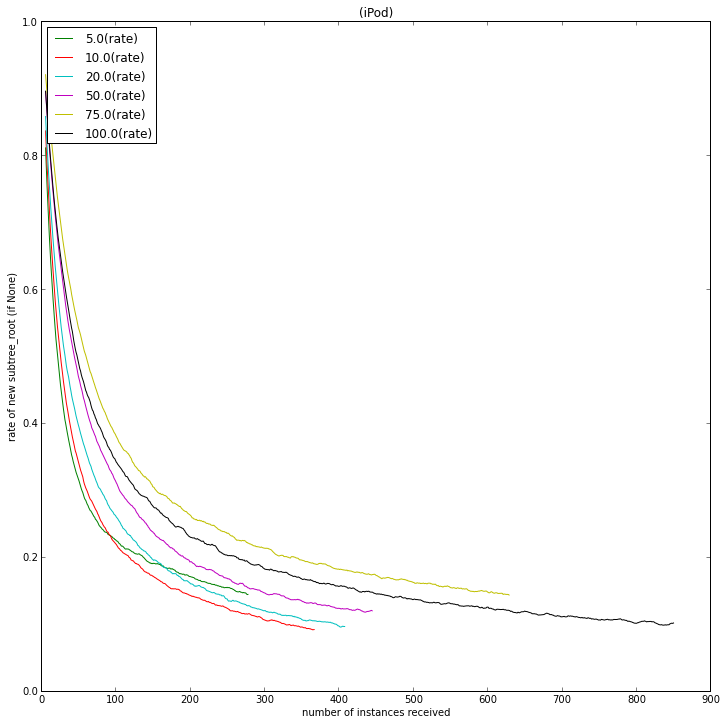
\includegraphics[width=0.7\columnwidth]{rate_new_category_over_time}
    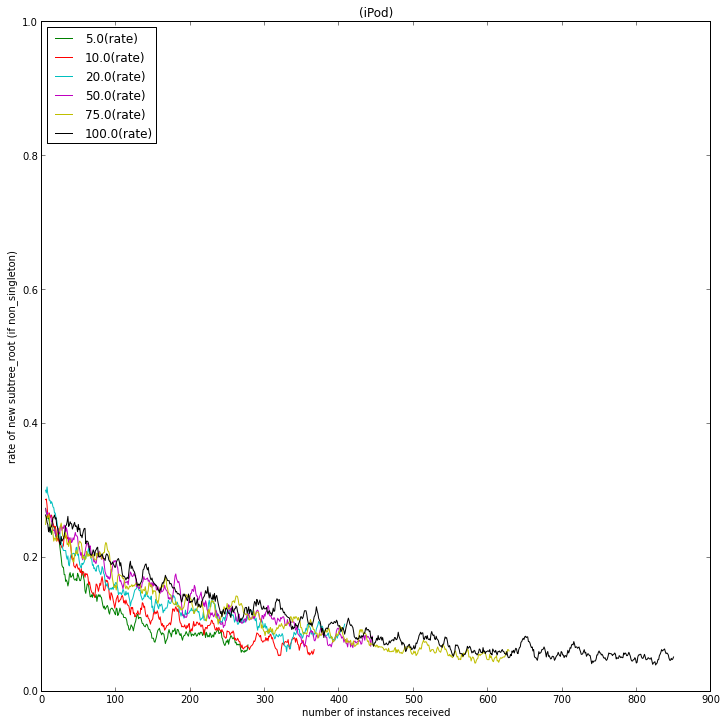
\includegraphics[width=0.7\columnwidth]{rate_new_ns_category_over_time}
    \caption{Rate of idea generation}
\end{figure}

We can perform a similar analysis for the number of new idea categories that arrive over time. As would be surmised from the previous graphs, we observe a similar pattern, which can also be modeled using a logarithmic model. As would also be expected, the number of new idea categories produced increases more slowly than the number of new ideas.

We see a very similar story with respect to differences in rates between conditions. The 5 and 10 conditions are virtually identical, while all other conditions are significantly different from one another.

Collectively, these results largely affirm hypotheses 1 and 2: The rate of new idea and new idea categories production quickly tapers off and tends toward zero over time. Furthermore, with a few exceptions, rates differ between conditions.



The third panel, which shows non-singleton categories over time, tells a distinctly different story from the others. While in the idea and category plots, the height-ordering of rates of generation between categories remains generally identical, there is a point of intersection and reversal in the non-singleton category plot at around the 30 instances point. Before this point, the lower conditions actually generate new categories at a \emph{faster} rate.

In lower conditions, brainstormers will quickly offer up big, popular, non-singleton categories. Beyond the inflection point, the category pool is saturated with these low-hanging fruit, and only brainstormers tasked with generating more ideas will find the smaller category. This is a more nuanced view of the tree node/instance quartiles in Section SEC; condition 5 brainstormers cover the spectrum of category sizes while condition 100 brainstormers pull from the smaller category trees in the forest.



The final measure, \emph{look-back equality}, is non-symmetrical and has meaning only in the context of a single brainstorming run. An instance \emph{a} is look-back equal to an \emph{earlier} instance \emph{b} if \emph{b} is in either \emph{a}'s idea node or any of \emph{a}'s parents, siblings, or children. This definition specifically identifies when a later instance in a run can be considered to have been influenced by earlier instance.


\subsubsection{Originality}

As our measure of originality, we use \emph{o-score}, introduced by Jansson and Smith \cite{jansson_design_1991}. An idea's o-score is $1 - p(idea)$, where $p(idea) = (number of instances of that idea)/(number of instances total)$. The o-score for category trees is similarly calculated. We will occasionally refer to the \emph{category o-score} of an idea. This simply refers to the o-score of the category tree to which that idea belongs.

\subsubsection{Uniqueness}


\subsection{Originality}

We measure differences in originality between conditions by examining the idea o-score and category o-score. The distributions of these scores are summarized in Figure FIG. The left panel compares idea o-score and the right compares category o-score.

\begin{figure}[h!]
    \centering
    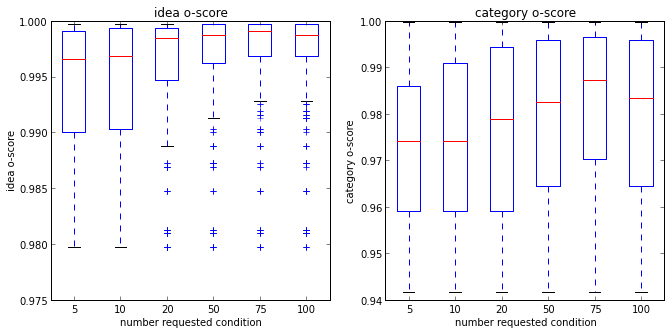
\includegraphics[width=0.9\columnwidth]{oscores_conditions}
\end{figure}

The more ideas requested, the more original the ideas produced. As suggested by the instance quartile range in section SEC, higher number conditions produce idea in trees with fewer instances, thus the high category o-score. We also see that these conditions produce \emph{ideas} with fewer instances.

As the originality rises, however, so does the number of outliers. To understand this phenomenon, we need to more closely observe the distribution of originality scores between not just conditions, but ordinal position in a brianstorming run.

Figure FIG provides this visualization. The upper panel gives the mean idea o-score as a function of ordinal position in all 100 condition brainstorming runs. The o-score for each ordinal position is the mean of all idea o-scores for that ordinal position in a run. Following this, the plot is further smoothed by making each point the mean of a sliding window of size 10 around its ordinal position. The bottom panel is a similar plot for category-oscore. To aid in interpretation, the first, second and third quartiles are also represented on the plot. The error bars are standard error.

\begin{figure}[h]
    \centering
    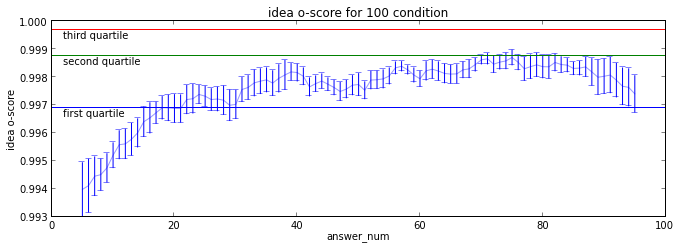
\includegraphics[width=0.9\columnwidth]{idea_oscore_order_100}
    \caption{Idea o-score as a function of order (100 condition)}
    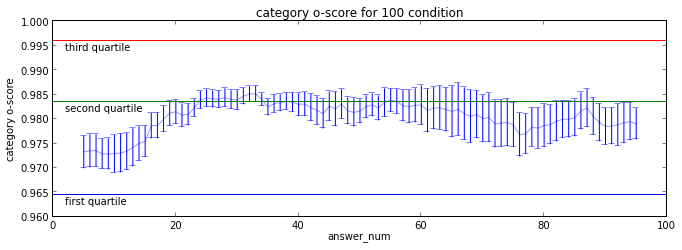
\includegraphics[width=0.9\columnwidth]{cat_oscore_order_100}
    \caption{Category o-score as a function of order (100 condition)}
\end{figure}

The only part of the originality score that falls outside the first and third quartiles is the beginning of the run. Participants in the higher numbered conditions generate more original ideas overall, but not until they have exceeded some threshold of common ideas. Figure FIG replicates figure FIG but across all conditions, and the same pattern of originality growth until an originality peak - around 20 ideas - is reached. Note that because of the additional HITs, there are far more examples of early-order ideas in the 5, 10 and 20 conditions than in the 50, 75, or 100, so this pattern is present without any dominating affect by the upper conditions.

\begin{figure}[h]
    \centering
    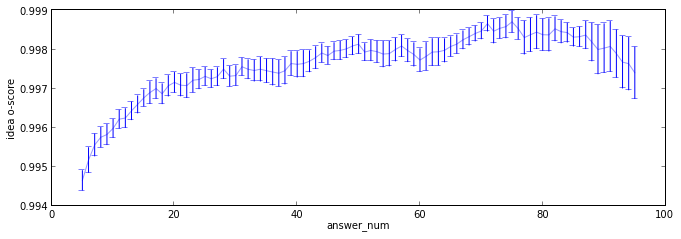
\includegraphics[width=0.9\columnwidth]{idea_oscore_order}
    \caption{Idea o-score as a function of order}
    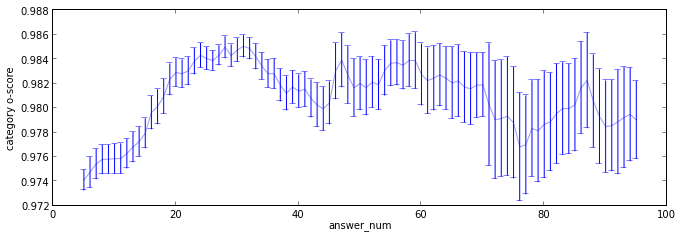
\includegraphics[width=0.9\columnwidth]{cat_oscore_order}
    \caption{Category o-score as a function of order}
\end{figure}

A similar, although less severe, pattern is observed for category o-score. There is a gradual increase in category originality until the 20 instance threshold is reached, at which point variance of the scores increases rapidly and no clear pattern is observable. This is explained by the relationship between common ideas and common categories. We expect that unoriginal ideas belong to unoriginal categories, as a high instance count for an idea increases the instance count for its category tree. However, we cannot make the inverse assumption, that a high originality idea belongs to a high originality category. Once the common idea are exhausted, then, there is no relationship between idea originality and category originality.

\subsubsection{Hypothesis 3}

This interpretation supports \textbf{Hypothesis 3:} There is a set of general, common ideas that make up the first several responses of every crowd brainstorming session, regardless of condition. We test this interpretation by constructing a set of the top 66 (5\%) most common ideas. If our intuition is correct, these ideas should be more likely to appear in the first 5 instances of a run than they are to appear in any of the following instances. We designate two Bernoulli variables. The first, defined by parameter $\theta_f$, represents the probability that an instance is in the common set given it is in the first five instances of a run. The second, defined by parameter $\theta_l$, is the probability that an instance is in the common pool given it is one of the \emph{last} (>5) instances in a run..

We fit these parameters using data from all runs with a total number of instances greater than 10. We chose this so that no run could contribute evidence to $\theta_f$ without also contributing to $\theta_l$. The resulting parameters were $\theta_f = 0.564$ (95\% HDI 0.517-0.611) and $\theta_l = 0.323$ (95\% HDI 0.303-0.342). This difference is significant, supporing the hypothesis that common ideas are over-represented in the early part of a brainstorming run, regardless of conditon.


\subsubsection{Hypothesis 6}

This threshold at 20 ideas brings us to \textbf{Hypothesis 6:} Ideas generated in the latter half of a brainstorming session are of higher originality than ideas generated in the former half. With our empirical evidence, we can instead test that ideas \emph{more than 20 instances into a brainstorming session} are more original than those in the first 20 instances, regardless of condition.

Test here...

\subsection{Riffing: We need to change the name of this}

At the level of the individual brainstorming run, we examine a new phenomenon related to uniqueness above. Within the SIAM model, \emph{riffing} (or \emph{clustering} as it is known in the work) occurs when a single participant activates a single image (analogous to a non-singleton category) and produces multiple ideas from that image under a fail state is reached and a transition is undergone to a new image. Unsurprisingly, we observed riffing activity in our data. An example of a single participant's riffed responses is given in Figure FIG. The second column is dark if the instance is a \emph{look-back equal} to any idea earlier in the run. The first column is dark if the instance is a \emph{source} instance, meaning it is the first in a chain of look-back equal instances. Riff chains can either be consecutive (as in the example), or separated with instances in between. The third column simply provides the text for that instance.

\begin{figure}[h]
    \centering
    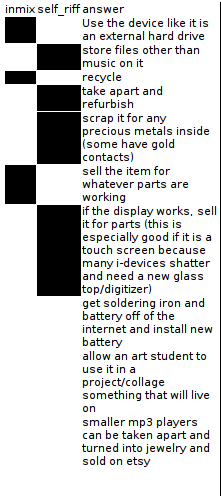
\includegraphics[width=0.5\columnwidth]{10_riff}
    \caption{Example of riffing in a size 10 run}
\end{figure}

The participant hits on the categories of using the device's hard drive for storage, recycling the device or its materials, and selling the device.  within these categories, they generate 2-3 ideas each. This is a fairly typical example of riffing. In larger conditions, it is common for participants to reach further back and return to an idea multiple time. Table TAB provides a summary of riffing between conditions.

\begin{table}
\begin{tabular}[h!]{r | l l l l l l l}
    \hline \hline \textbf{condition} & 5 & 10 & 20  \\ \hline \hline
    \% riffs & 13.65 & 19.28 & 25.17  \\
    source instances & 10.58 & 12.92 & 15.01 \\
    riffs per source & 1.29 & 1.49 & 1.68 \\
    median length of consecutive chain & 2 & 2 & 2 \\
    median distance to previous in chain & 1 & 2 & 2 \\
    median distance to first in chain & 2 & 3 & 5 \\ \hline \hline
    \textbf{condition} & 50 & 75 & 100 \\ \hline \hline
    \% riffs & 39.6 & 32.81 & 42.81 \\
    source instances & 19 & 17.19 & 18.13\\
    riffs per source & 2.08 & 1.91 & 2.36\\
    median length of consecutive chain & 2 & 2 & 2\\
    median distance to previous in chain & 7 & 10 & 5\\
    median distance to first in chain & 16.5 & 18 & 26.5 \\
    \end{tabular}
    \caption{Riffing statistics by condition}
\end{table}

The higher the number of instances requested, the more participants riff on their old ideas. Similarly, upper conditions use more of their ideas as sources for riffing, and riff more times on each of those ideas. The primary surprise is that they do not riff more consecutively. The median length of a consecutive riff chain remains low across conditions. This leaves us with the image of a participant in the upper conditions searching through their old ideas for something to build upon one instance at a time.

Another outlier of note is the relatively short median distance to a previous idea in a chain for the 100 condition. Participants in the 100 condition may feel more pressure to remix, and return to earlier ideas more quickly than those in the 50 or 75 conditions.

\subsubsection{Hypothesis 4}

Riffing activity is analogous to idea production within an image as described by Nijstad and Stroebe's SIAM model \cite{nijstad_how_2006}. Thus, we should expect to confirm their hypothesis, \textbf{Hypothesis 4}, that \emph{an idea from one semantic category should more often by followed by an idea from the same category than expected by random chance}.

To test this, we modelled the probability of any category being followed by the same category with a Bernoulli distribution. Each instance not the first in its run was a trial. If the instance was in the same category tree as the previous instance, the trial was a pass. Otherwise, it was a failure. The Bernoulli $\theta$ was 0.156 (95\% HDI 0.143 - 0.170).

The most common category tree in our data set, \emph{music player}, represents only 5.65\% of instances. This is well below the 0.143 lower-bound of HDI. Thus, we accept the hypothesis that an instance follows a previous instance in the same category with greater probability than is explained by random chance.

\subsection{Completion Time}

As another aspect of how participants complete brainstorming runs, we are interested in the time spent on each response. The first, second and third quartiles for each condition are given in boxplots in figure FIG. The whiskers extend to 1.5 times the inner quartile range. Surprisingly, we see many instances taking up to 28018382ms (7.78 hours) to complete.

\begin{figure}[h]
    \centering
    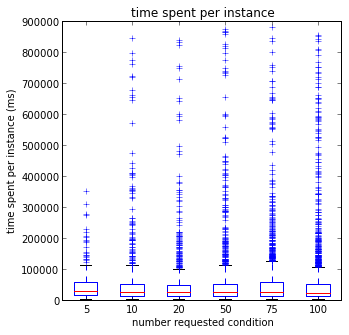
\includegraphics[width=0.9\columnwidth]{time_spent_condition}
    \caption{Time spent per instance}
\end{figure}

Either our participants were exceedingly concerned with crafting their responses, or there is another influence at work. Figure FIG gives the mean time spent on an instance by order, separated by condition. Most of the highly variant response times take place early in the brainstorming run. This suggests that at least one participant accepted a brainstorming task, took an initial stab at instances, and then left the task for up to 8 hours before continuing. Beyond this, we might expect to see time spent per instance go up as participants have to dig deeper to find responses, but no such effect is consistently observed.

\begin{figure}[h]
    \centering
    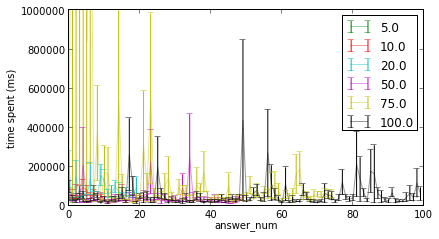
\includegraphics[width=0.9\columnwidth]{time_spent_order}
    \caption{Time spent per instance}
\end{figure}

\subsubsection{Hypotheses 5}

The Nijstad and Stroede \cite{nijstad_how_2006} model also provides \textbf{Hypothesis 5}: \emph{idea generation when changing semantic categories should take longer than idea generation within categories}. An examination of the distribution of data for time spent per instance suggested a log-normal distribution, with the frequency of occurances quickly rising until a peak was reached, followed by a gradual drop-off. As with previous tests, we used the Stan package for Bayesian inference [CITE]. We fit, two models: $t_w = \text{lognormal}(\mu_w, \sigma_w)$ for within-category idea generation and $t_b = \text{lognormal}(\mu_b, \sigma_b)$ for between-category idea generation, where the $t$ parameter in each model represents the time spent generating an instance.

\begin{figure}[h]
    \centering
    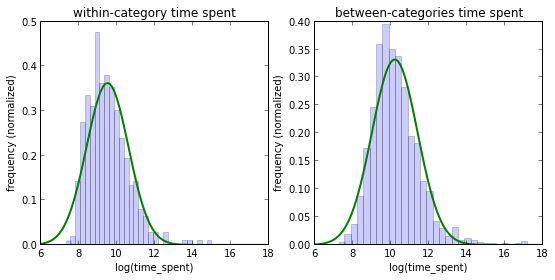
\includegraphics[width=0.9\columnwidth]{hyp5_comparison}
    \caption{Time spent to generate an instance}
\end{figure}

The resulting fit models are shown in Figure FIG, overlapping the log-space histograms for observed values. The mean for the within-category condition was 9.5 in log space (13.4 seconds, 95\% HDI 9.4-9.6), while the mean for the between-categories condition was 10.2 (27.0 seconds, 95\% HDI 10.2-10.3). The variances were 1.1 (3 seconds) and 1.2 (3.3 seconds) respectively. These difference were both sigificant. Within-category instance generation took on average 12.6 seconds less than between-categories. This is consistent with the findings of Nijstad and Stoebe, who reported differences of 6-12 seconds.
